\documentclass{article}
\usepackage{amsmath,epsfig,rotating}

\begin{document}

\begin{flushleft}
{\sc \Large Control Systems - Project Report} \hfill \\ $ $ \\
\medskip
Name: Mian Inshaullah  \\
Enrollment Number: 18PWCSE1721\\
Section: A \\
\today
\end{flushleft}


\section{Problem which is considered}
\noindent A hard disk is a data storage device. It uses magnetic storage system with electronic hardware to access the data. The electronic circuit consists of a dc motor. A dc motor has the following state space:\\
\begin{equation}
\begin{bmatrix} \dot{\theta}\\  \dot{\Theta} \\ \dot{i}\end{bmatrix}
= \begin{bmatrix}
0 & 1 & 0 \\
0 & \frac{-b}{J} & \frac{k}{J} \\
0 & \frac{k}{L} & \frac{-R}{L}  \end{bmatrix}
\begin{bmatrix} \theta\\  \Theta \\ i \end{bmatrix} +
\begin{bmatrix}
0 \\
0 \\
\frac{1}{L}  \end{bmatrix}
 u 
\end{equation}\vskip10pt

\begin{equation}
y(t)=\begin{bmatrix}
1 & 0 & 0
\end{bmatrix}
\begin{bmatrix} \theta \\  \Theta \\ i \end{bmatrix}
\end{equation}




\\
\noindent a. Use J = 3.2, b = 3.5, k = 0.0274, R = 4, and L = 2.75; Check the stability of the system using all methods that \\
\\
b. Simulate the unstable system and show that its response is unstable \\\\
c. Compute the controllability matrix for the system. If the system is controllable, place the controller eigenvalues at (-14, -33, -33) and observer eigenvalues at a location which is faster than the controller \\\\
d. Simulate the stable system and show its response \\\\
e. Design a PID Controller and compare it with response obtained from part d\\ \\
f. Compute the steady state errors before and after designing controller\\ \\
g. Design a tracking controller for step tracking of amplitude 5u(t) and ramp tracking of 5tu(t)\\ \\
% This command is done for extra space
\vskip30pt

\section{Solution}
In this report, we address the the above problem and explain each subproblem in detail.


\subsection{State-space Representation of the System}
The state-space representation of the system can be written as follows:

\begin{equation}
\begin{bmatrix} \dot{\theta}\\  \dot{\Theta} \\ \dot{i}\end{bmatrix}
= \begin{bmatrix}
0 & 1 & 0 \\
0 & -1.0938 & 0.0086 \\
0 & 0.01 & -1.4545  \end{bmatrix}
\begin{bmatrix} \theta\\  \Theta \\ i \end{bmatrix} +
\begin{bmatrix}
0 \\
0 \\
0.3636  \end{bmatrix}
 u 
\end{equation}

\begin{equation}
y(t)=\begin{bmatrix}
1 & 0 & 0
\end{bmatrix}
\begin{bmatrix} \theta \\  \Theta \\ i \end{bmatrix}
\end{equation}



\subsection{Stability analysis of the system}
In this section, we analyze the stability of the system. The stability can be checked using different ways namely eigenvalues, step response, poles, root locus and RH-stability criteria. For our case, the system is of 3rd order and therefore there will be three eigen values. Let $\lambda_1$ and $\lambda_2$ and $\lambda_3$ denote the eigenvalues of the system. The values of eigenvalues can be written as follows:
\begin{equation} \lambda_1 = 0,   \lambda_2 = -1.4545,  \lambda_3 = -1.0935 \end{equation}
\vskip10pt
\noindent The eigenvalues of the system were computed using \textit{eig(A)} matlab function
\vskip10pt
\noindent As we can see one of the eigenvalue is zero while all others are negative, which indicates the system is marginally stable. Next, we verify the same fact by observing the poles of the system. Let $p_1$ and $p_2$, and $p_3$ denote the poles of the system. The values for poles are as follows:
\begin{equation} p_1 = 0 ,  p_2 = -1.0935 ,  p_3 =-1.4545  \end{equation}
The poles of the system were computed using the \textit{roots(denum)} matlab function. 
\vskip10pt

We observe here again that one of the poles is zero while all others are negative, which indicates the system is marginally stable. \vskip100pt

\noindent Next, we verify the same fact by seeing the step-response of the system. The step-response of open-loop system is shown in Figure 1.

\begin{figure}[h!]
\centering
\includegraphics[scale=0.5]{Step_Response.jpg}
\caption{Plot of step response.}
\end{figure}

From Figure 1, we can do the following analysis: \\
\begin{equation}\begin{aligned}
\%OS & = Undefined\\
T_r & = Undefined\\
T_s & = Undefined\\
Peak Value & = \infty \\
Final Value & = \infty\end{aligned} \notag \end{equation}

\vskip120pt
\noindent Next, we construct a Routh-Hurwitz table to check the stability of the system.
\begin{table}[h] \begin{center}
\scalebox{1.5}{%
\begin{tabular}{|l|c|l|} \hline
$s^3$  & 1 & 1.591\\ \hline
$s^2$ & 2.548 & 0 \\ \hline
$s^1$  & $-\frac{1}{2.548}\times\begin{vmatrix} 1 & 1.591\\ 2.548 & 0 \end{vmatrix} $ = $ 1.5910$ & 0 \\ \hline
$s^0$  & $-\frac{1}{-1.5910}\times\begin{vmatrix} 1.591 & 0\\ 1.591 & 0 \end{vmatrix}= 0$ & 0 \\ \hline
\end{tabular}}\end{center}
\end{table}

\noindent As there are no sign changes in the first column, the system is stable.
\vskip30pt

\noindent Next we can analyze the Root locus Plot of the system. The Root Locus Plot of the system is as below:
\begin{figure}[h!]
\centering
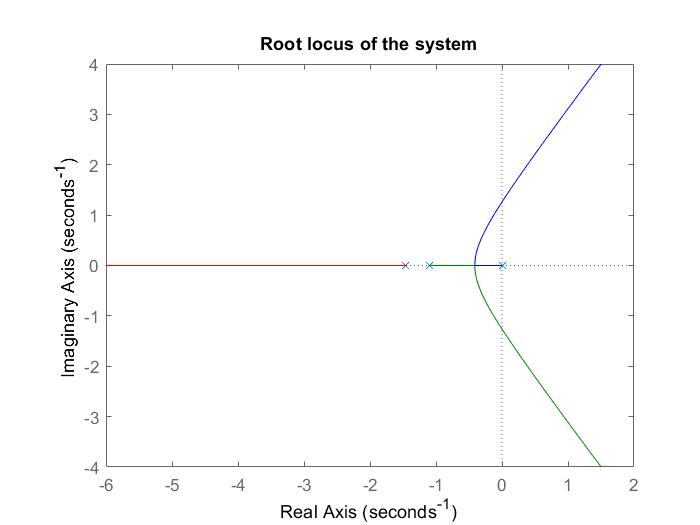
\includegraphics[scale=0.5]{root_locus.jpg}
\caption{Plot of Root Locus.}
\end{figure}
\vskip10pt
\noindent As we can see, at gain k = 0, System is Marginally Stable


\subsection{Controllability analysis of the system}
\noindent The System is marginally stable. We shall consider it as unstable because it has an unbounded output as seen in Figure 1 and Figure 2. To design a controller for this system, we need to ensure the system passes all the prerequisites. \\

\noindent 
\begin{itemize}
\item The System should be unstable
\item Rank of Matrix P should equal to n of the Matrix A. \\
\end{itemize}

\noindent Let us Check if it passes the Controllability test. \\
\vskip10pt
\noindent Compute the Controllability Matrix P of Matrix A and Matrix B using the following function: \begin{equation} P = ctrb(A, B) \end{equation}\vskip10pt
\noindent Our Matrix P is as follows:
\begin{equation}
\begin{bmatrix}
\
0 & 0 & 0.0031 \\
0 & 0.0031 & -0.0079 \\
0.3636 & -0.5289 & 0.7694  \end{bmatrix}
\end{equation}
\vskip10pt
\noindent Next compute the rank of Matrix P using the following function: 

\begin{equation}
Ctrb rank = rank(P)
\end{equation}
\noindent The rank is as follows:
\begin{equation}
 Ctrbrank = 3
\end{equation}
\vskip20pt
\noindent As rank of Matrix P is same as matrix A, we conclude that the system passes controllability test. Since the system is controllable, we place controller eigen values at (-14, -33, -33)
\pagebreak
\subsection{Observability analysis of the system}
\noindent The System is controllable. However, we need to ensure it is observable because matrix C is not an Identity Matrix. Therefore, we should compute the observability matrix. To design an observer for this system, we need to ensure the system passes all the prerequisites.\\

\begin{itemize}
\item The System should be unstable
\item Matrix C should not be an Identity Matrix
\item Rank of Matrix Q should be equal to n of the Matrix A
\end{itemize}

\noindent Let us Check if it passes the Controllability test. \\
\vskip10pt
\noindent Compute the Controllability Matrix P of Matrix A and Matrix B using the following function: \begin{equation} P = obsv(A, C) \end{equation}\vskip10pt
\noindent Our Matrix Q is as follows:
\begin{equation}
\begin{bmatrix}
\
1 & 0 & 0 \\
0 & 1 & 0\\
0 & -1.0938 & 0.0086  \end{bmatrix}
\end{equation}
\vskip10pt
\noindent Next compute the rank of Matrix Q using the following function: 

\begin{equation}
Obsv rank = rank(Q)
\end{equation}
\noindent The rank is as follows:
\begin{equation}
 Obsv rank = 3
\end{equation}
\vskip20pt
\noindent As rank of Matrix Q is same as matrix A, we conclude that the system passes controllability test. Since the system is controllable, we place controller eigen values at (-15, -34, -34)
\pagebreak
\subsection{Controller Design for the system}
\noindent Now that we know that our system is both observable and controllable, we shall design an Observer based State Feedback controller and PID Controller. \\

\noindent To design our Controller, we first place the poles using the acker function as below: 
\\
\begin{center}
\textit{observer = [-15, -34, -34]\\
controller  = [-14, -34, -34]\\
L = acker(A', C',  observer)'\\
K = acker(A, B,  controller)\\}
\end{center}

\\
Output:
\begin{equation}
L = \begin{bmatrix}
80.4517 \\
1.9694 * 10^3 \\
1.6756 * 10^6 \end{bmatrix}
\end{equation}
\vskip15pt
\begin{equation}
K = 
\begin{bmatrix}
4.8965*10^6 & 6.1879*10^5 & 212.9922 
\end{bmatrix}
\end{equation}
\vskip10pt

\noindent Now that we have our desired K and L matrices, we can design an Observer-based State Feedback Controller. 

\pagebreak
\section{Results and Discussions}
\subsubsection{Observer based State Feedback Controller}

Schematic of our Observer based State Feedback Controller is as below:

\begin{figure}[h!]
\centering
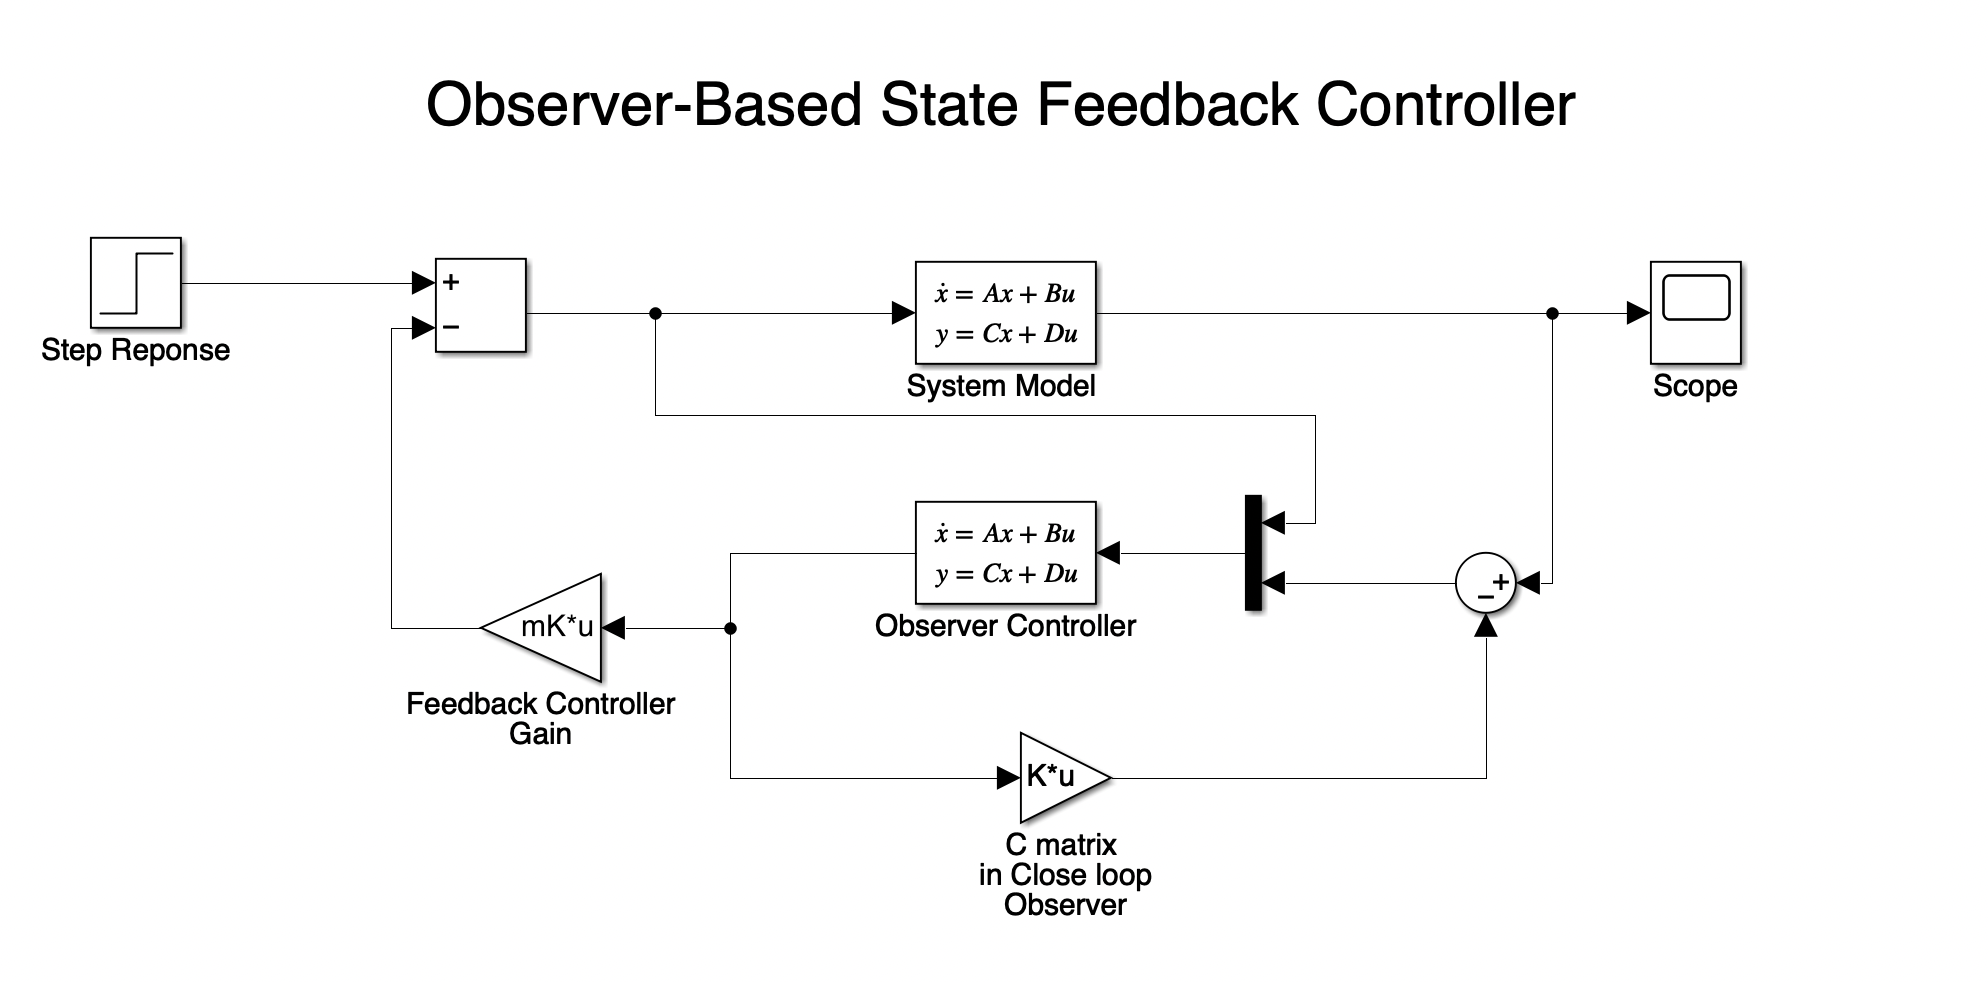
\includegraphics[scale=0.3]{ObserverbasedSFC.jpeg}
\caption{Schematic of  Observer based State Feedback Controller.}
\end{figure}
\vskip30pt

\subsubsection{Response of Observer based State Feedback Controller}
Response of Observer based State Feedback Controller is as follows: 
\begin{figure}[h!]
\centering
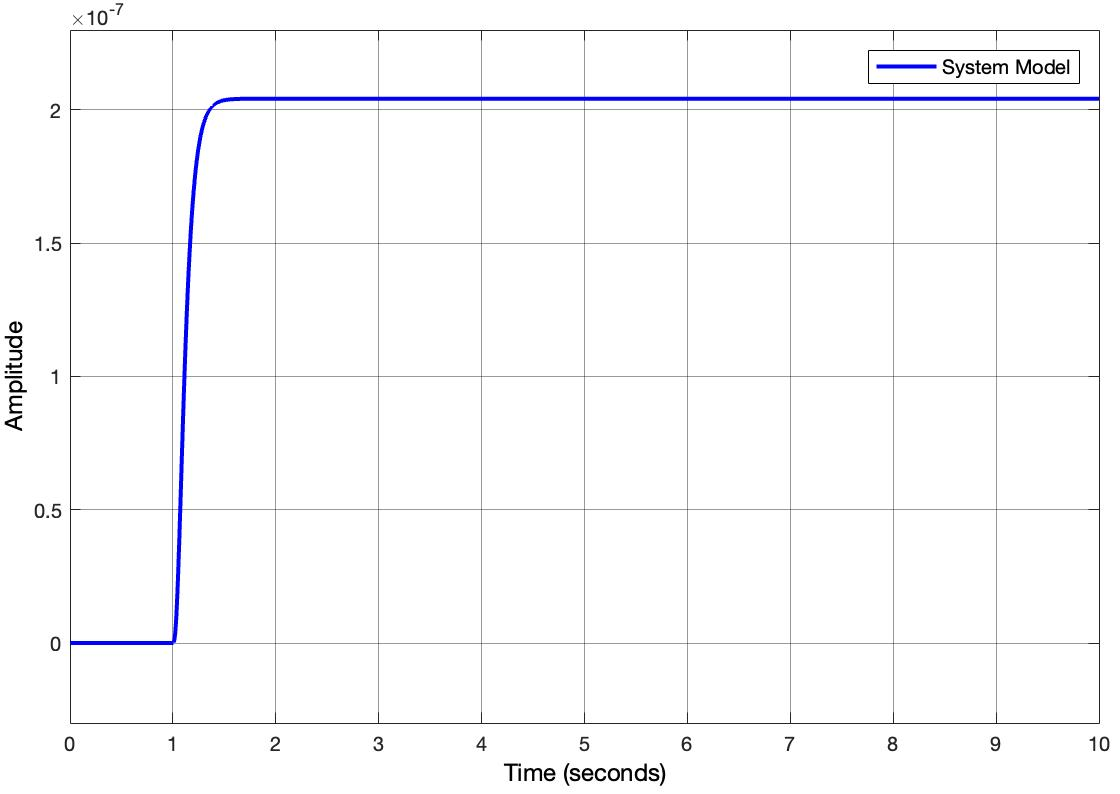
\includegraphics[scale=0.25]{ObserverbasedSFC_response.jpg}
\caption{Plot of Response of  Observer based State Feedback Controller.}
\end{figure}
\vskip10pt

\subsubsection{Analysis of Response from Observer based State Feedback Controller}
\begin{equation}\begin{aligned}
\%OS & = 0\\
T_r & = 0.3580 \;seconds \\
T_s & = 0.3580 \;seconds\\
Peak Value & = \frac{2.0417}{10^7} \\
Final Value & = \frac{2.0417}{10^7} \end{aligned} \notag \end{equation}\vskip150pt

\subsubsection{PID Controller for Observer based State Feedback Controller}
Schematic of our PID Controller is as below:

\begin{figure}[h!]
\centering
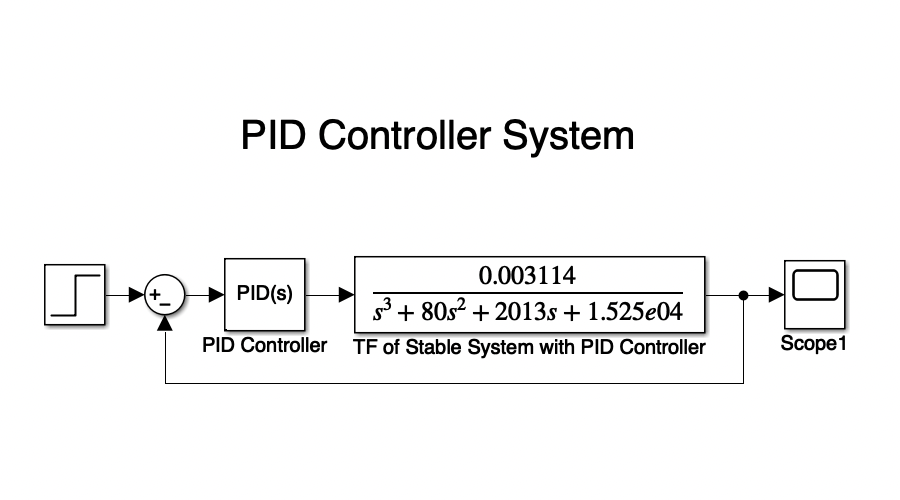
\includegraphics[scale=0.6]{PID_Model.png}
\caption{Schematic of  PID Controller.}
\end{figure}
\vskip30pt

\subsubsection{Response of PID Controller for Observer based State Feedback Controller}
Response of PID Controller for Observer based State Feedback Controller is as follows: 
\begin{figure}[h!]
\centering
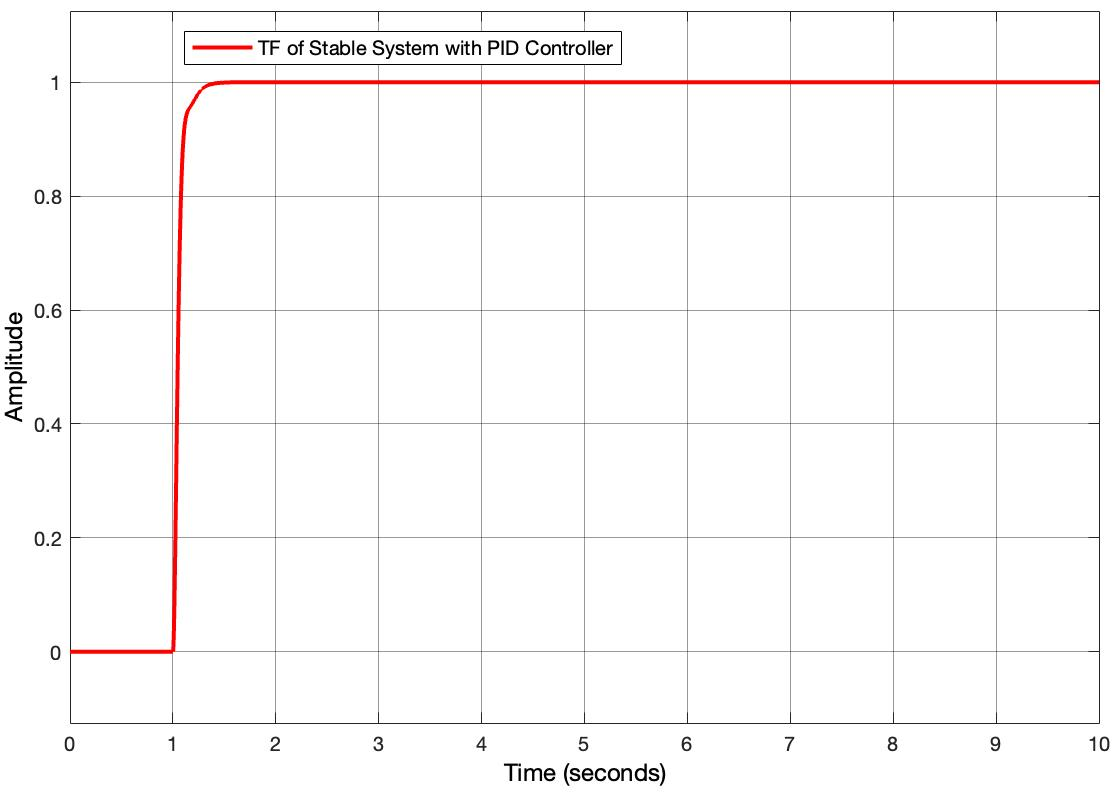
\includegraphics[scale=0.25]{pid_response.jpg}
\caption{Plot of Response of PID Controller for Observer based State Feedback Controller.}
\end{figure}
\vskip10pt

\subsubsection{Analysis of Response from Observer based State Feedback Controller}
\begin{equation}\begin{aligned}
\%OS & = 0\\
T_r & = 0.2257 \;seconds \\
T_s & = 0.2257 \;seconds\\
Peak Value & = 1 \\
Final Value & = 1 \end{aligned} \notag \end{equation}\pagebreak
\subsubsection{Comparison of  PID Controller with Controlled System }
Here's a comparison of the Outputs of all the systems. 
\vskip10pt
\begin{figure}[h!]
\centering
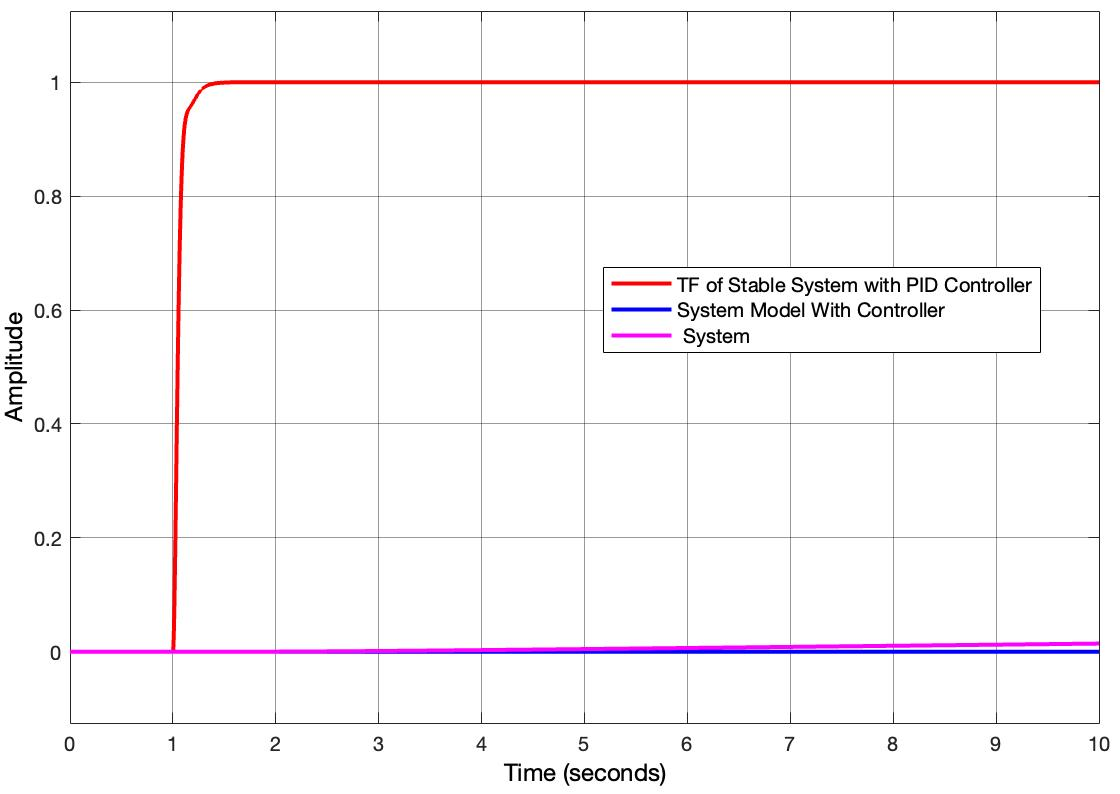
\includegraphics[scale=0.25]{Comparison.jpg}
\caption{Comparison of Step Responses of Observer based State Feedback Controller, PID Controller, and Marginally Stable System.}
\end{figure}

\subsubsection{Steady State Errors}

\begin{itemize}
\item Steady State Error before the controller:
\begin{itemize}
\item Infinity or Undefined because system output is unbounded. 
\end{itemize}

\item Steady State Error after Observer-based Feedback Controller
\begin{itemize}
\item  \begin{equation}
1 - \frac{2.0417}{10^7}\approx 1
\end{equation}
\end{itemize}

\item Steady State Error after PID Controller
\begin{itemize}
\item \begin{equation}
1 - 1 = 0 
\end{equation}
\end{itemize}
\end{itemize}
\begin{itemize}
\item Steady State Error for Ramp Input after Controller
\begin{itemize}
\item Infinity because system is Type 0
\end{itemize}
\item Steady State Error for Parabolic Input after Controller
\begin{itemize}
\item Infinity because system is Type 0
\end{itemize}
\end{itemize}

\subsubsection{Tracking Controllers}
\begin{figure}[h!]
\centering
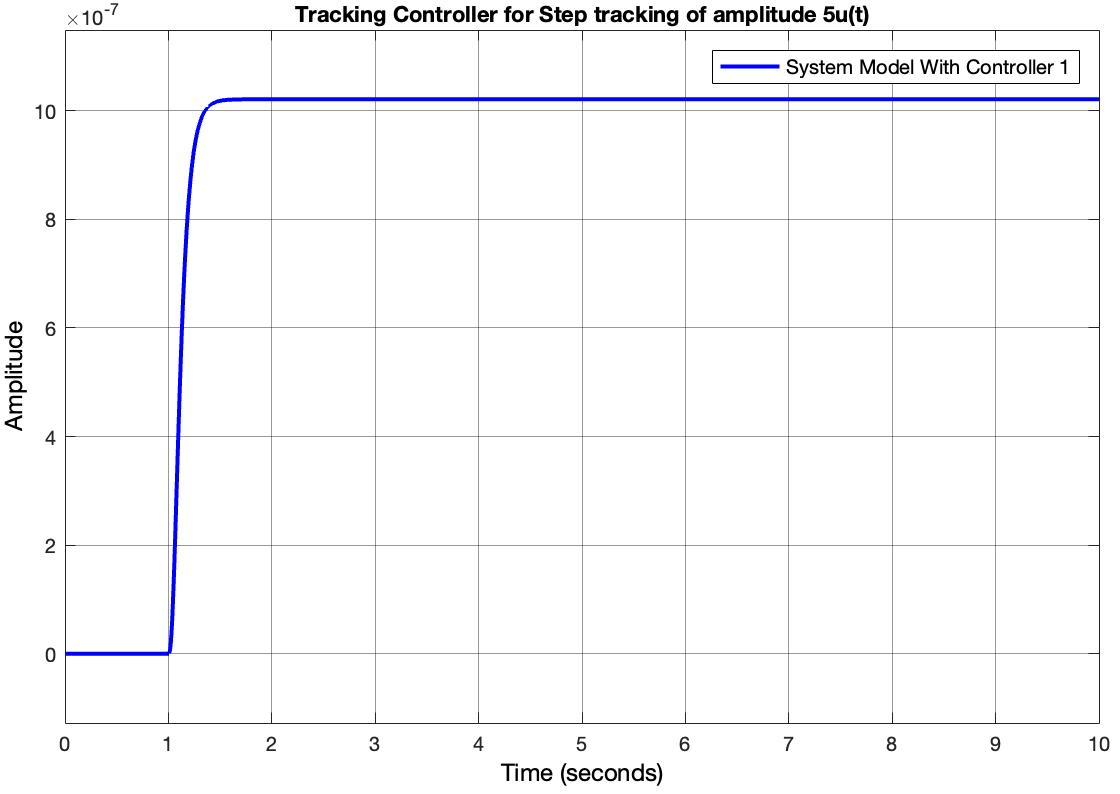
\includegraphics[scale=0.25]{Steptracking.jpg}
\caption{Plot of Step Tracking of amplitude 5u(t).}
\end{figure}



\begin{figure}[h!]
\centering
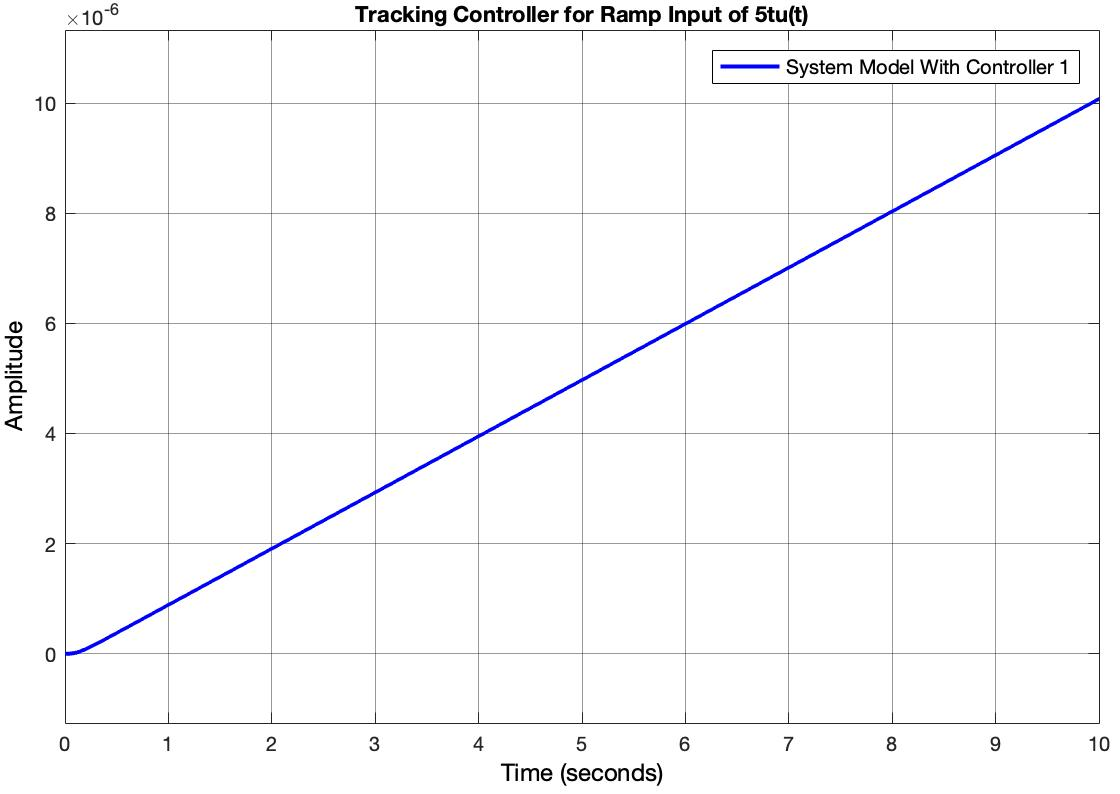
\includegraphics[scale=0.25]{TrackingControllerResponse.jpg}
\caption{Plot of Ramp Tracking of amplitude 5tu(t).}
\end{figure}


\end{document} 